\chapter{Shanghai}
\section*{14 septembre 2015}
Beaucoup de sites internet comme Google, Twitter ou Facebook sont bloqués en Chine, heureusement le blog est accessible ! \newline
 Après un court vol de 3h j'atteris à Shanghai. Première impression, des infrastructures très modernes partout, des immeubles très hauts, pas une ambiance vraiment chinoise \newline
 \newline
\centerline{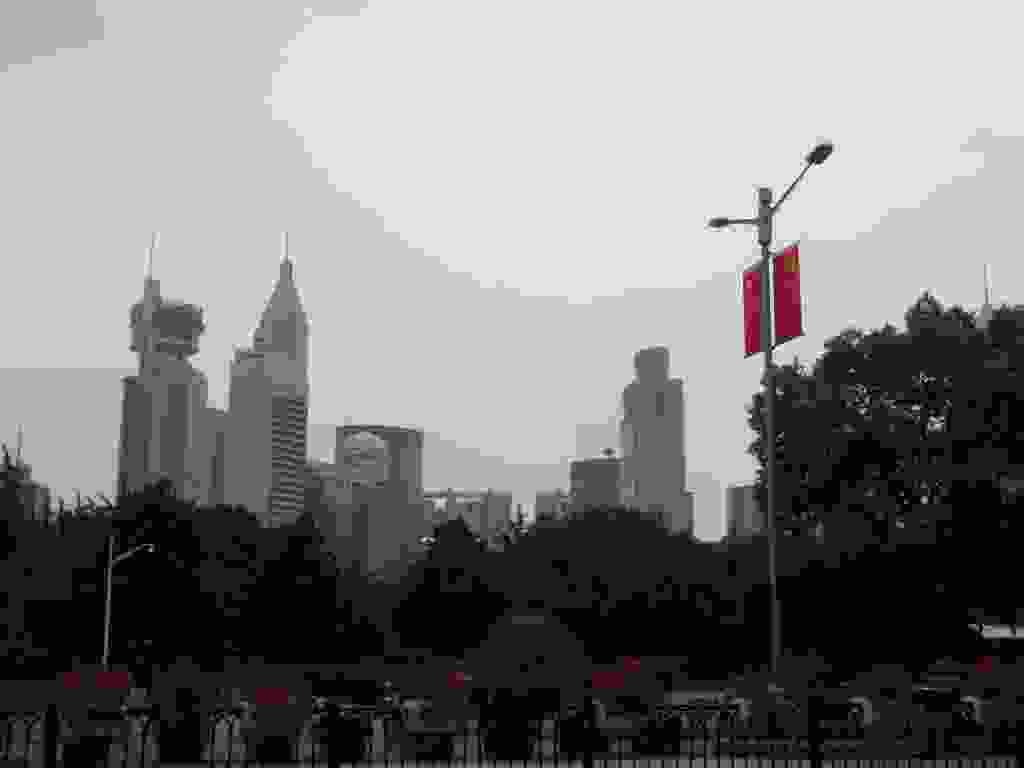
\includegraphics[width=\mywidth]{../wp-content/uploads/2015/09/P8316550-1024x768.jpg} } 
 \newline
 Pas de vélo ici, le métro est pratique et sécurisé, il y a même une vérification des sacs à l'entrée \newline
 \newline
\centerline{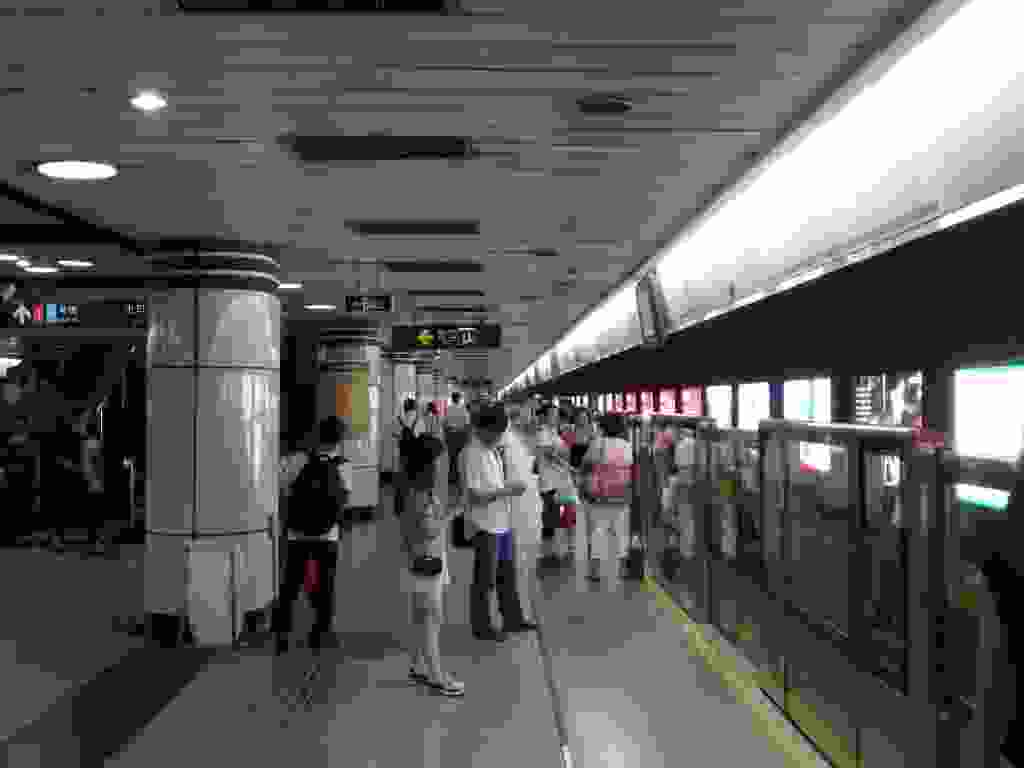
\includegraphics[width=\mywidth]{../wp-content/uploads/2015/09/P9016606-1024x768.jpg} } 
 \newline
 Je suis hébergé dans le quartier de la concession francaise, agréable avec beaucoup d'arbres \newline
 \newline
\centerline{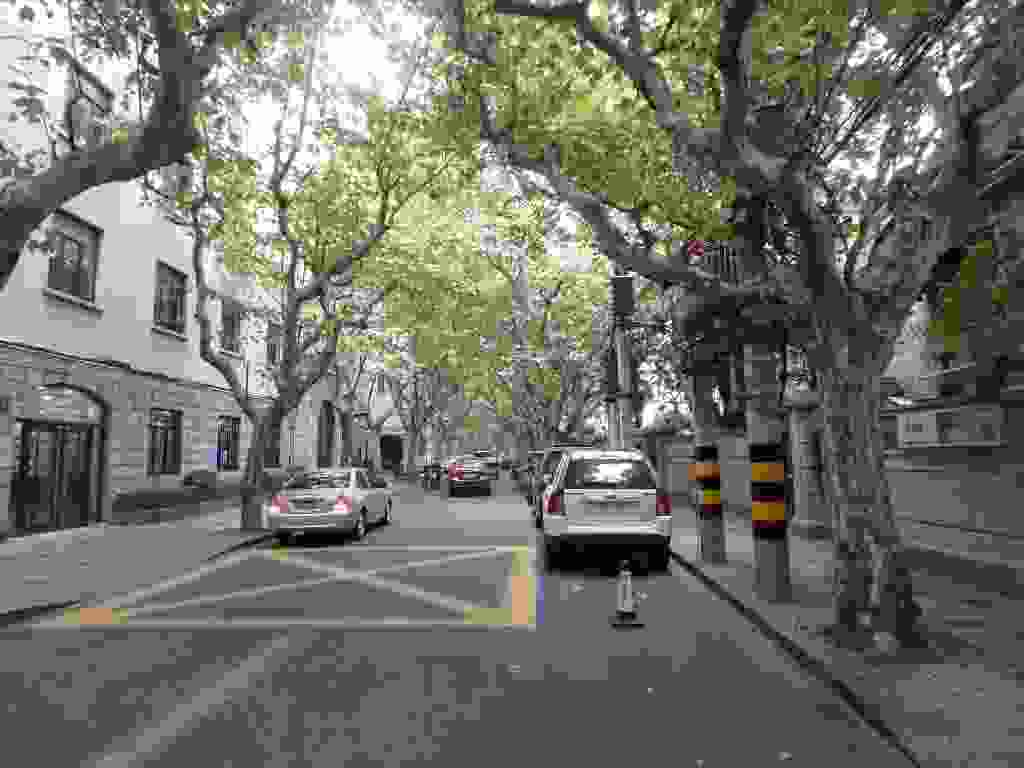
\includegraphics[width=\mywidth]{../wp-content/uploads/2015/09/P8316529-1024x768.jpg} } 
 \newline
 Je commence par une balade dans le parc Fu Xing le matin. \newline
 \newline
\centerline{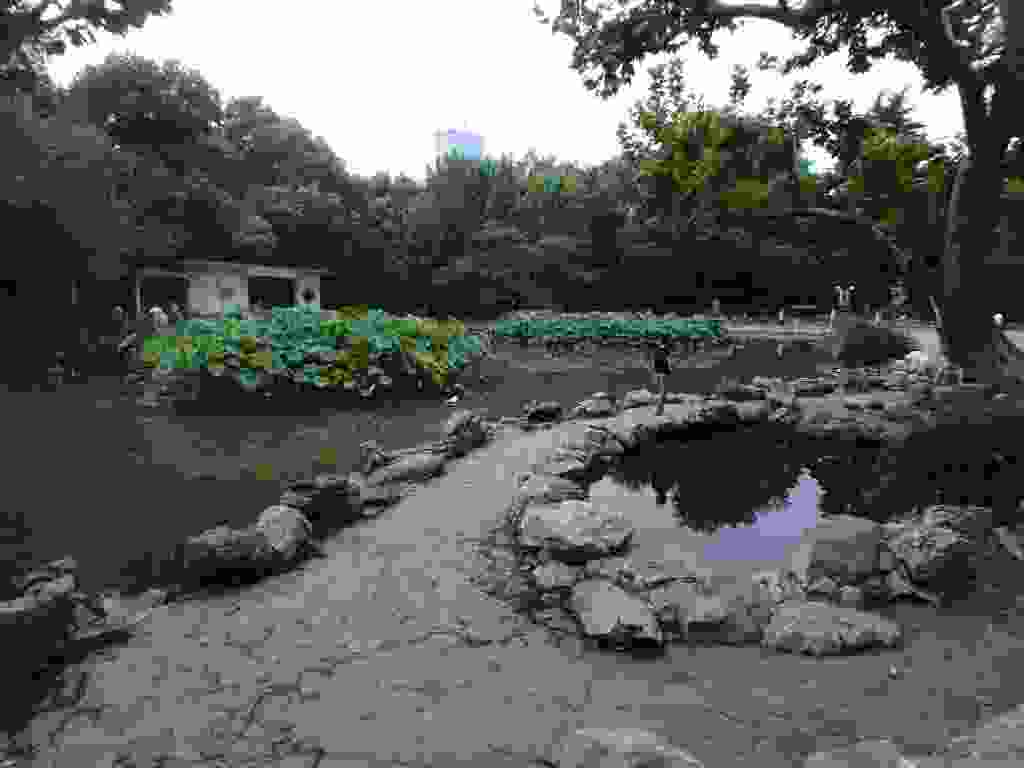
\includegraphics[width=\mywidth]{../wp-content/uploads/2015/09/P8316533-1024x768.jpg} } 
 \newline
 Les gens s'adonnent à tous types d'activités \newline
 \newline
\centerline{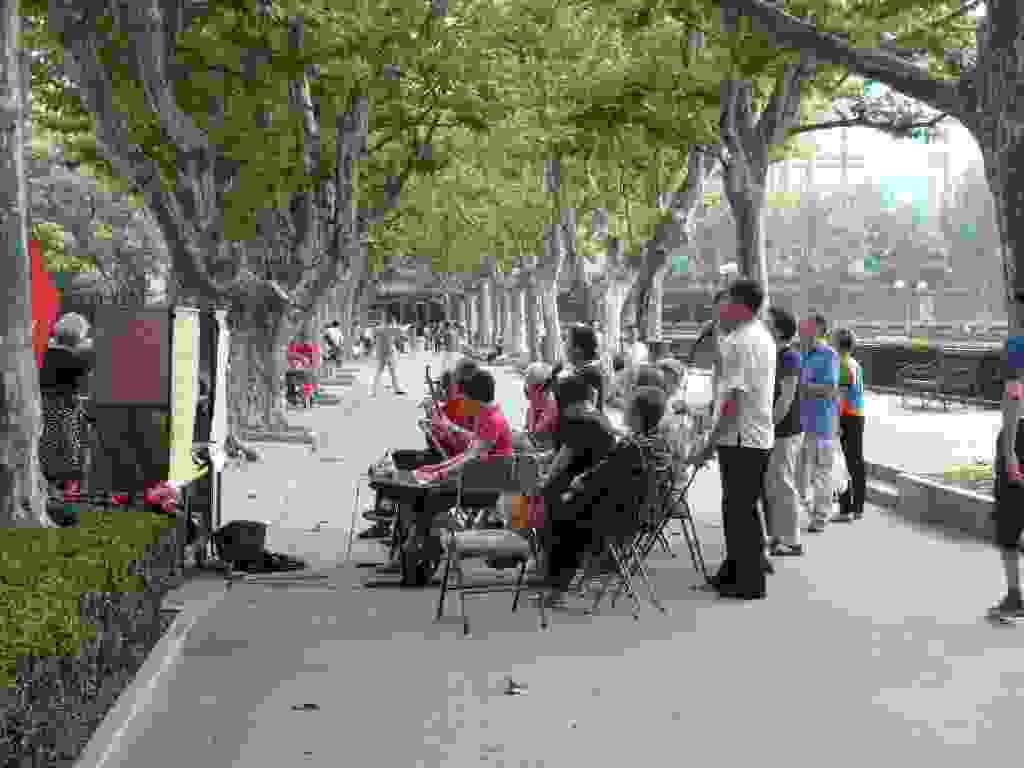
\includegraphics[width=\mywidth]{../wp-content/uploads/2015/09/P8316536-1024x768.jpg} } 
 \newline
 \newline
\centerline{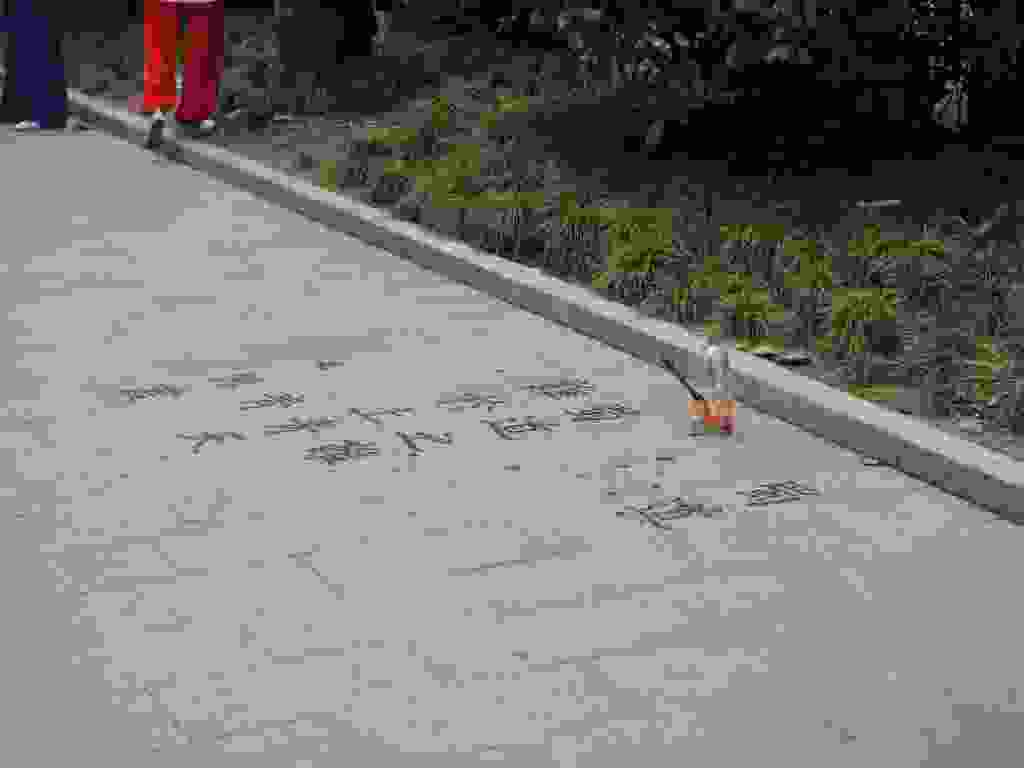
\includegraphics[width=\mywidth]{../wp-content/uploads/2015/09/P8316538-1024x768.jpg} } 
 \newline
 \newline
\centerline{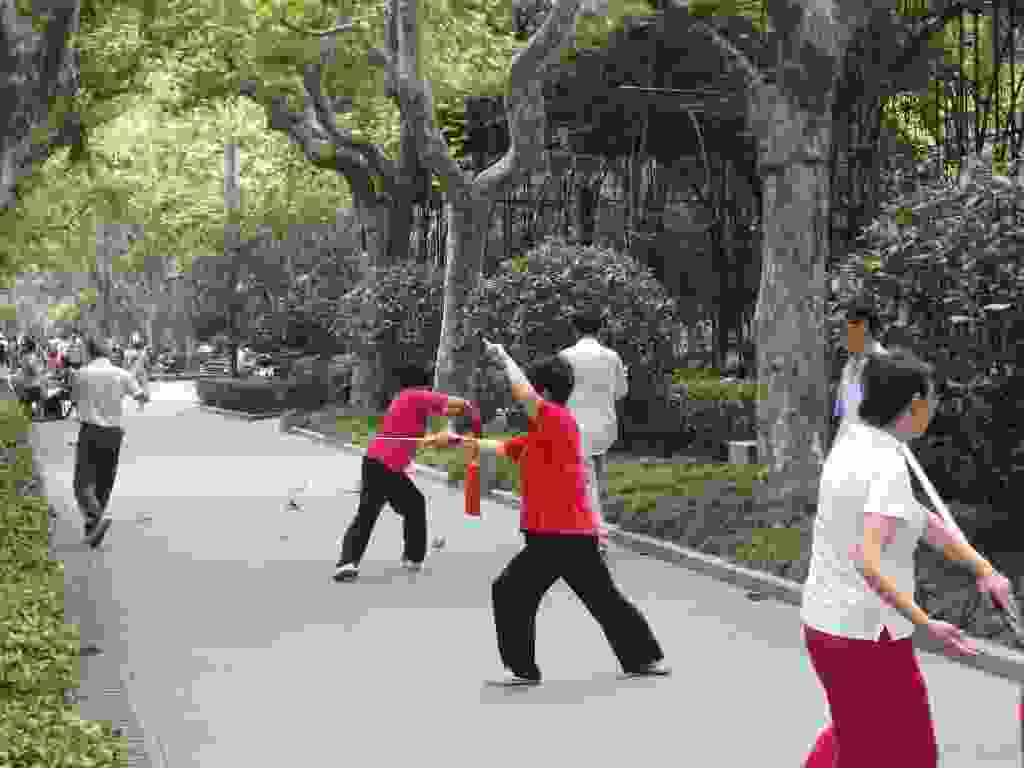
\includegraphics[width=\mywidth]{../wp-content/uploads/2015/09/P8316539-1024x768.jpg} } 
 \newline
 \newline
\centerline{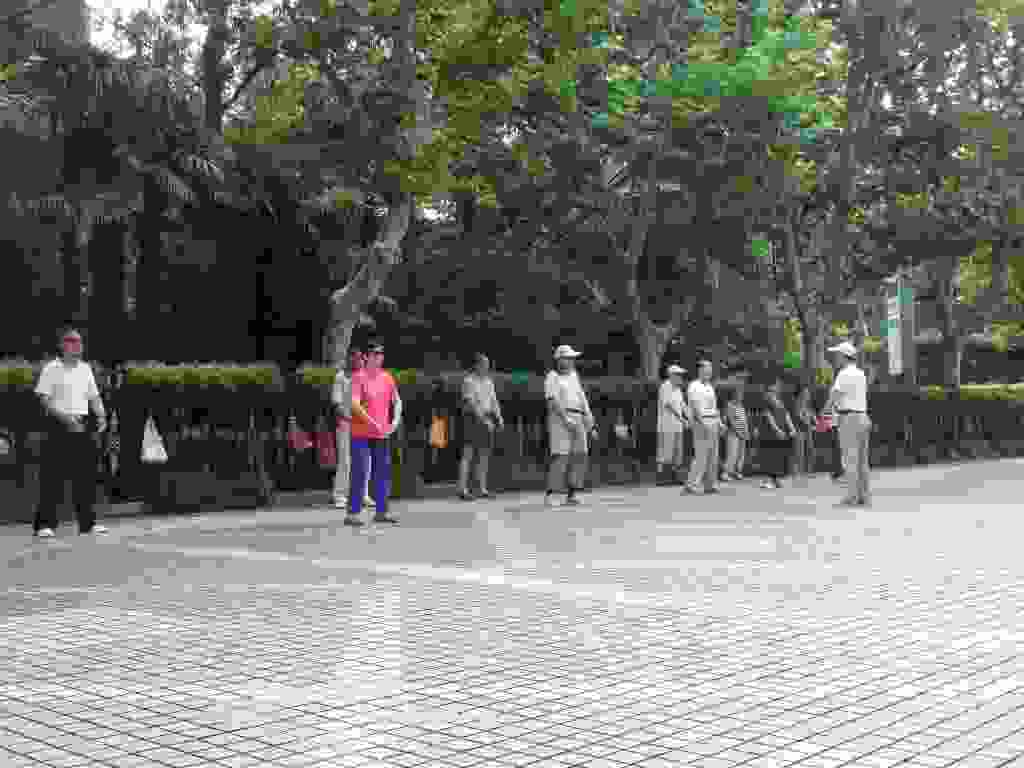
\includegraphics[width=\mywidth]{../wp-content/uploads/2015/09/P8316541-1024x768.jpg} } 
 \newline
 \newline
\centerline{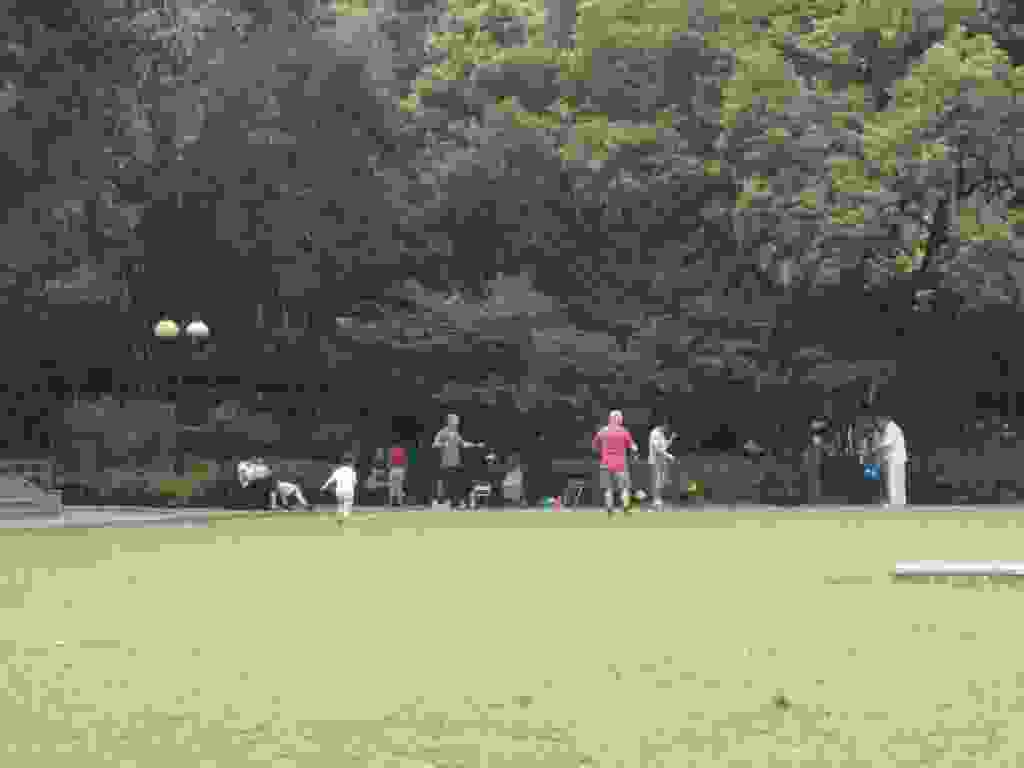
\includegraphics[width=\mywidth]{../wp-content/uploads/2015/09/P8316542-1024x768.jpg} } 
 \newline
 People's Square, la place principale de Shanghai \newline
 \newline
\centerline{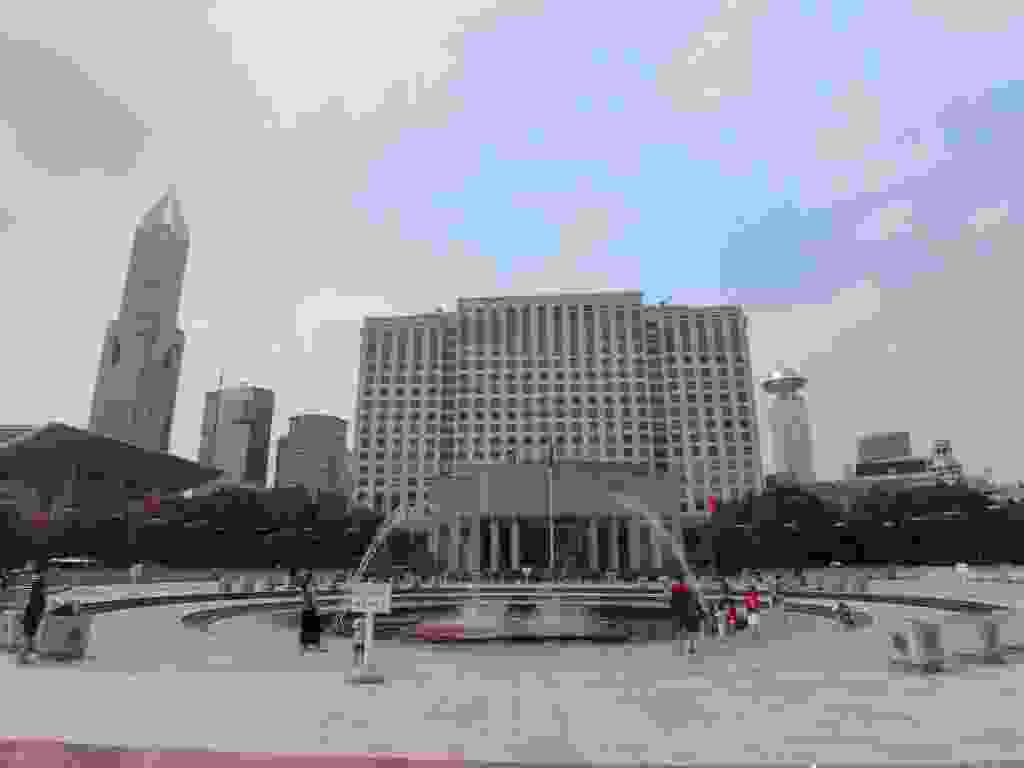
\includegraphics[width=\mywidth]{../wp-content/uploads/2015/09/P8316552-1024x768.jpg} } 
 \newline
 C'est là que se trouve le Shanghai Museum \newline
 \newline
\centerline{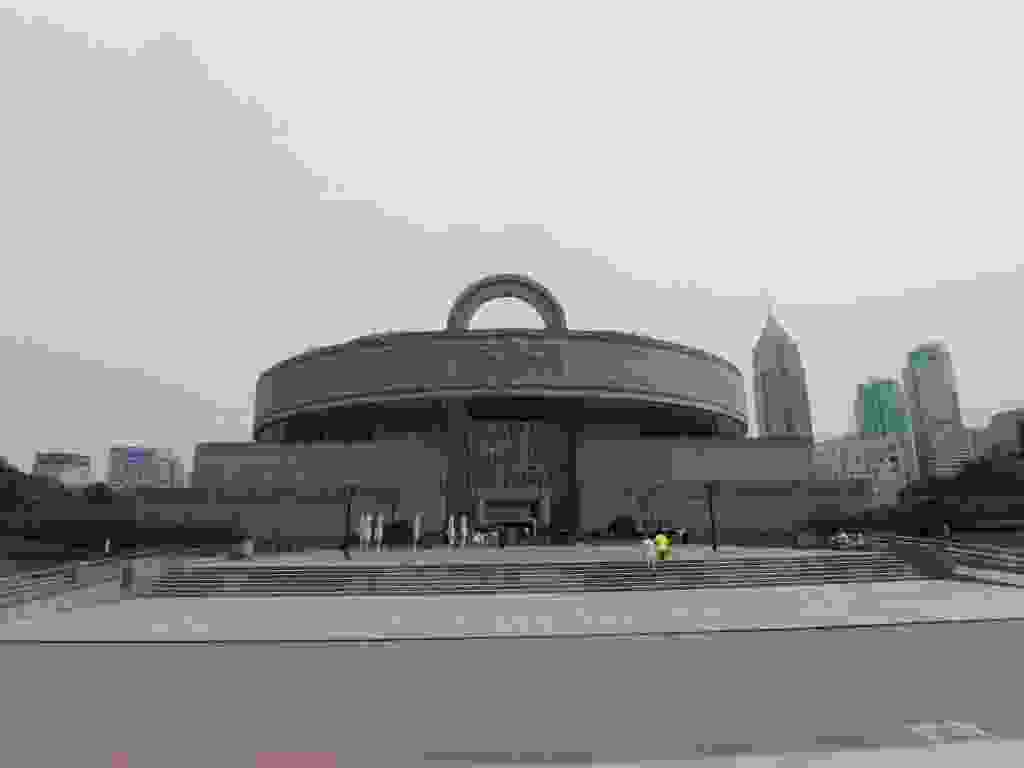
\includegraphics[width=\mywidth]{../wp-content/uploads/2015/09/P8316553-1024x768.jpg} } 
 \newline
 \newline
\centerline{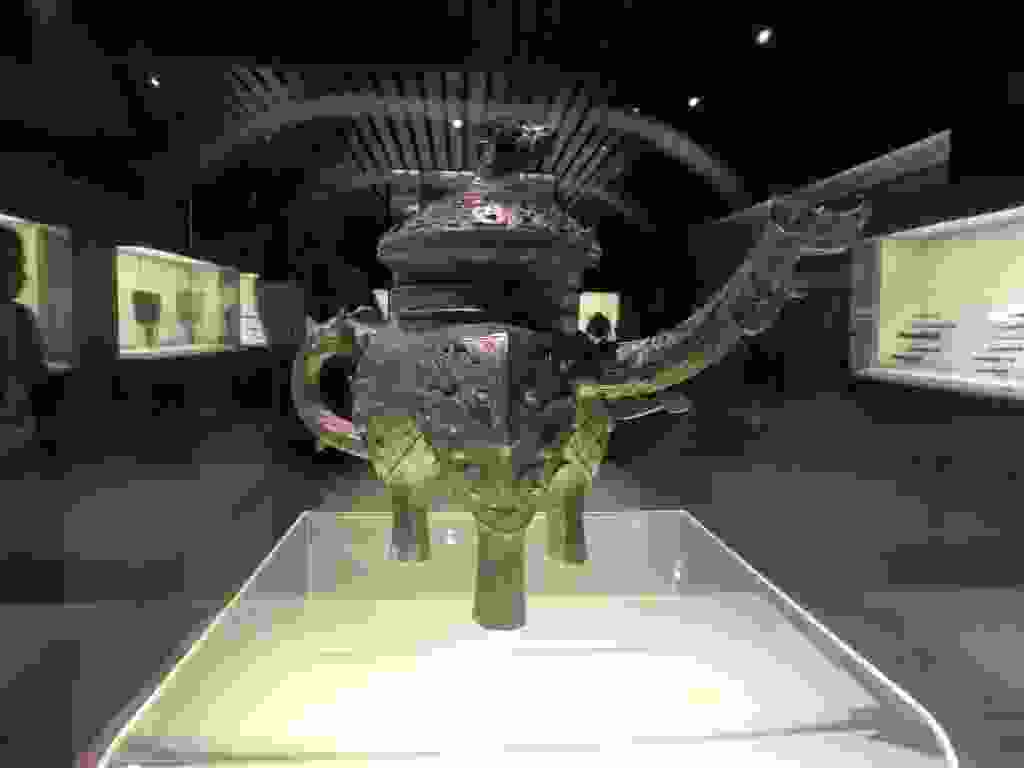
\includegraphics[width=\mywidth]{../wp-content/uploads/2015/09/P8316556-1024x768.jpg} } 
 \newline
 \newline
\centerline{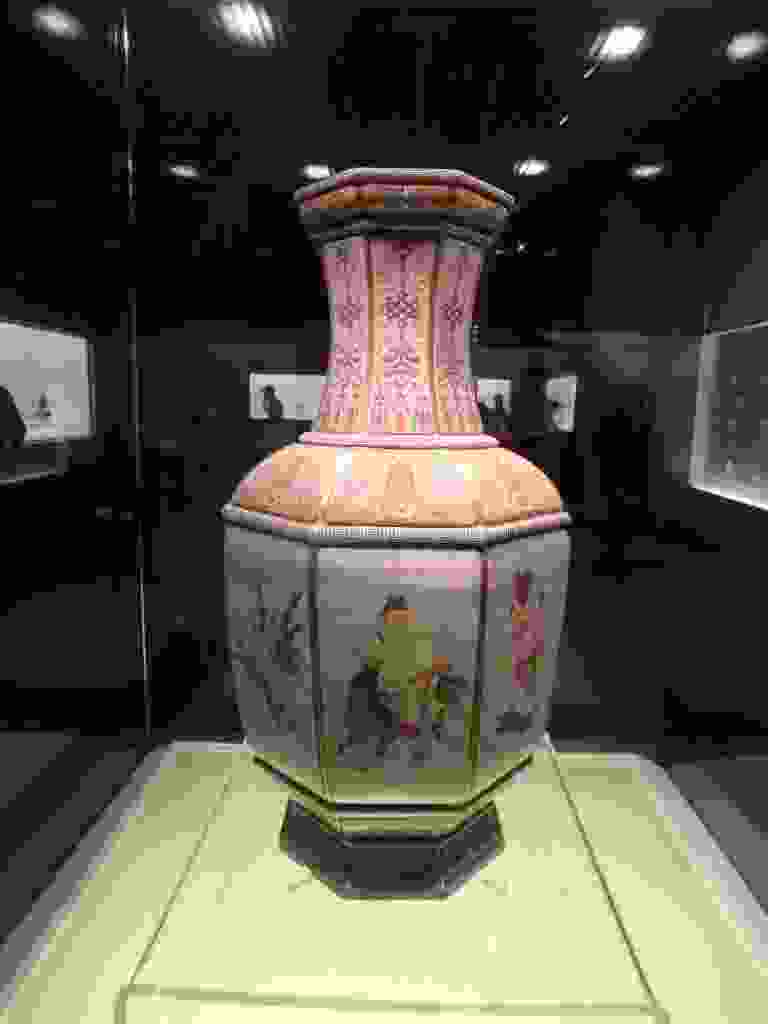
\includegraphics[width=\mywidth]{../wp-content/uploads/2015/09/P8316558-e1441267394556-768x1024.jpg} } 
 \newline
 \newline
\centerline{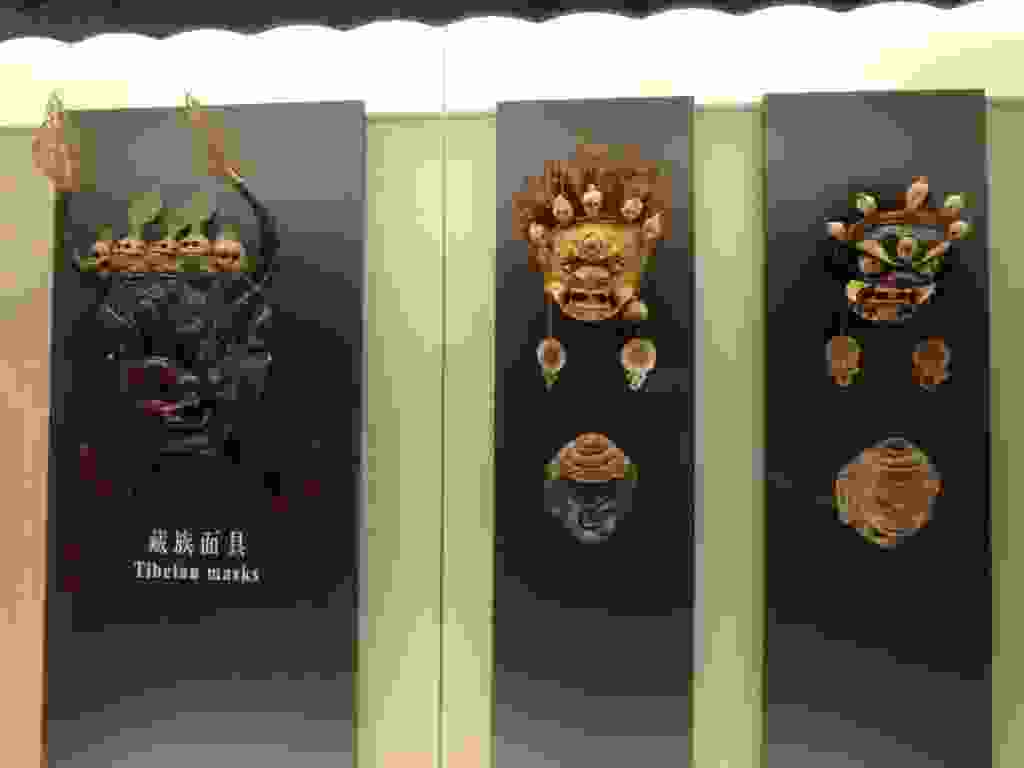
\includegraphics[width=\mywidth]{../wp-content/uploads/2015/09/P8316560-1024x768.jpg} } 
 \newline
 \newline
\centerline{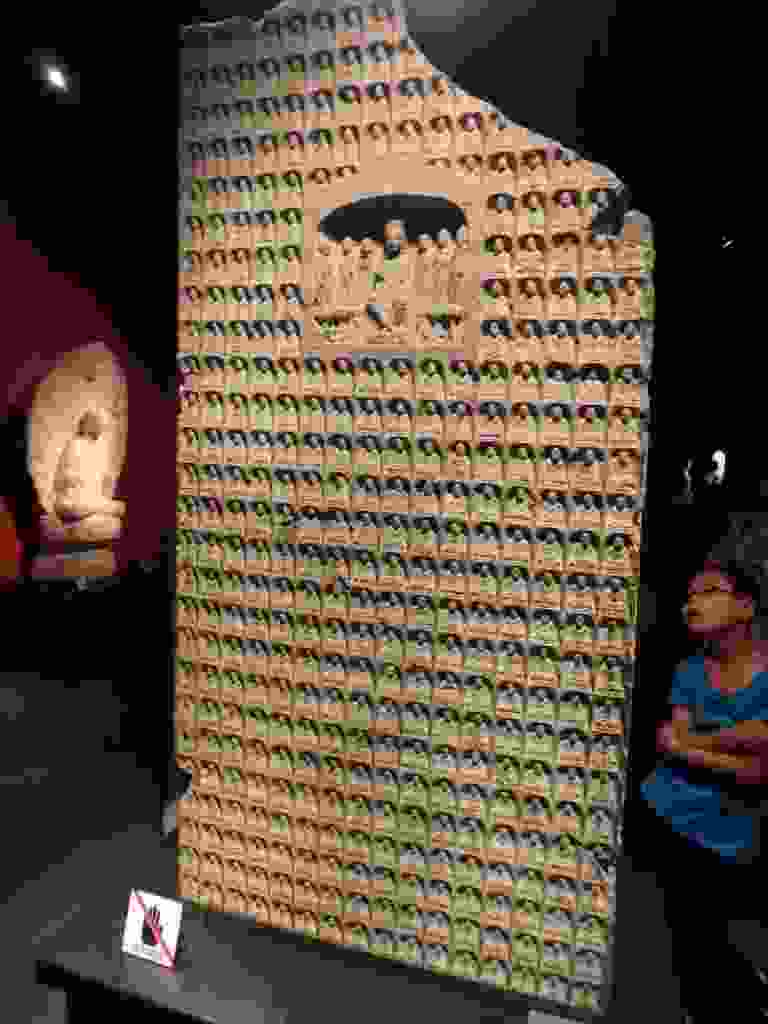
\includegraphics[width=\mywidth]{../wp-content/uploads/2015/09/P8316561-e1441455299605-768x1024.jpg} } 
 \newline
 La Nanjing Road, rue touristique avec des boutiques \newline
 C'est dans cette rue que j'observe 2 fois la tentative d'arnaque classique de Shanghai : un groupe de jeunes chinois très sympatiques et parlant bien anglais viennent discuter, après un bon moment ils me proposent de venir boire un thé. Comme j'étais prévenu je ne les ai pas suivi mais le principe est ensuite de faire payer une addition exhorbitante pour le thé. \newline
 \newline
\centerline{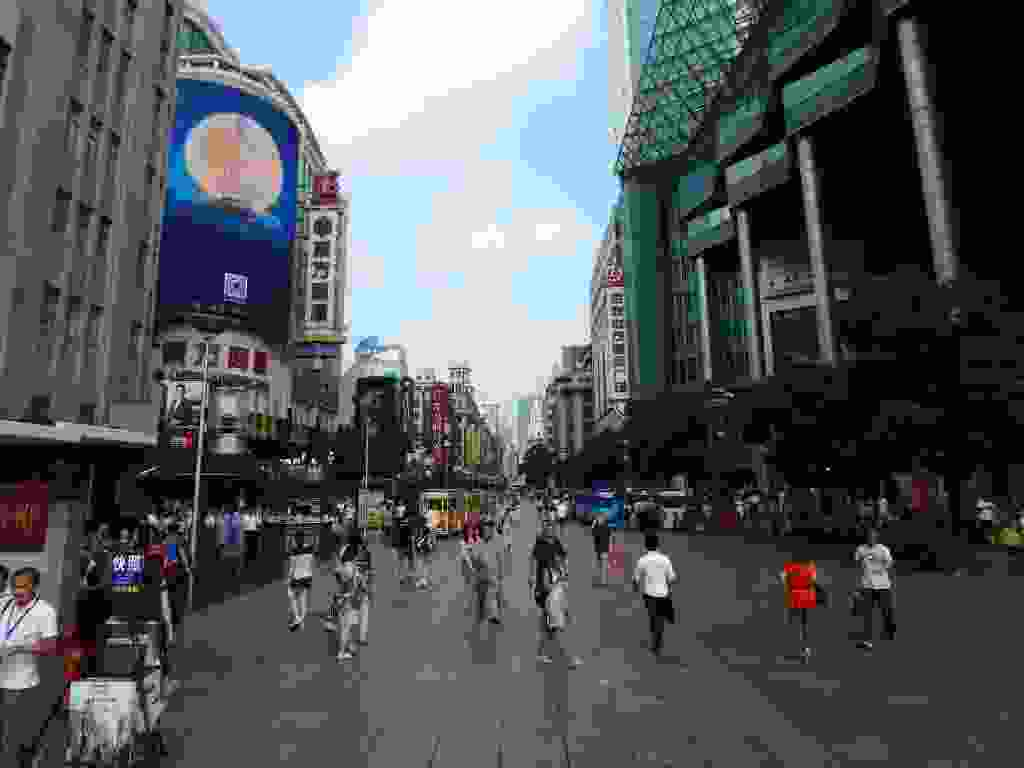
\includegraphics[width=\mywidth]{../wp-content/uploads/2015/09/P8316564-1024x768.jpg} } 
 \newline
 La rue se termine sur The Bund avec la vue la plus célèbre de Shanghai \newline
 \newline
\centerline{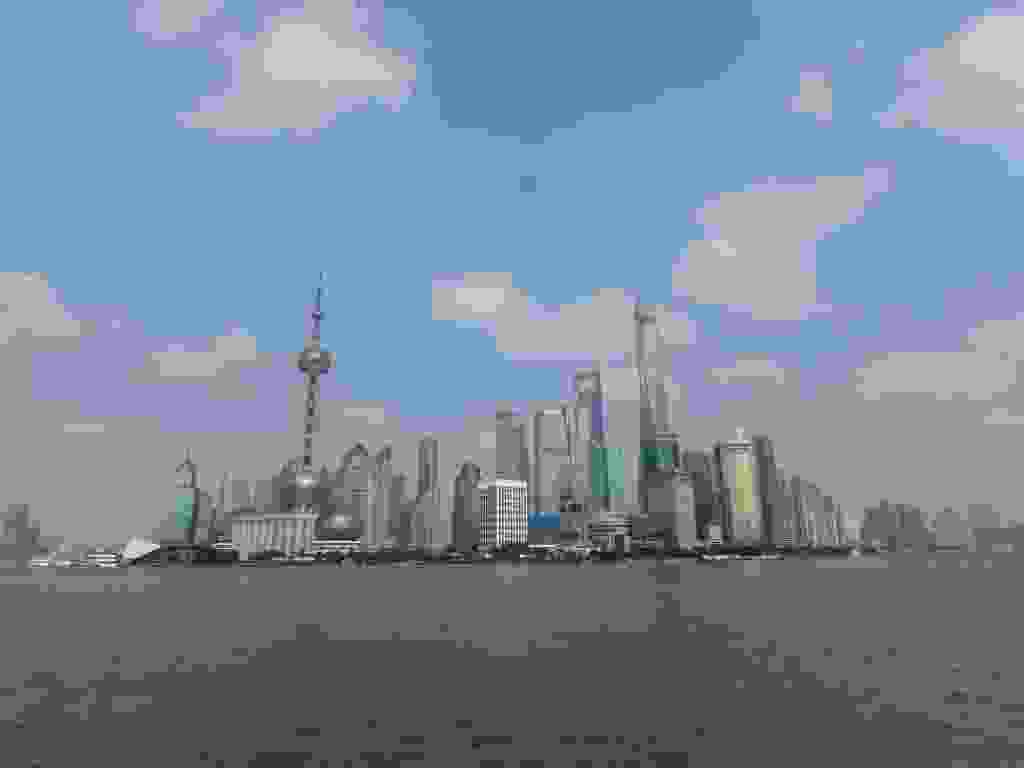
\includegraphics[width=\mywidth]{../wp-content/uploads/2015/09/P8316565-1024x768.jpg} } 
 \newline
 \newline
\centerline{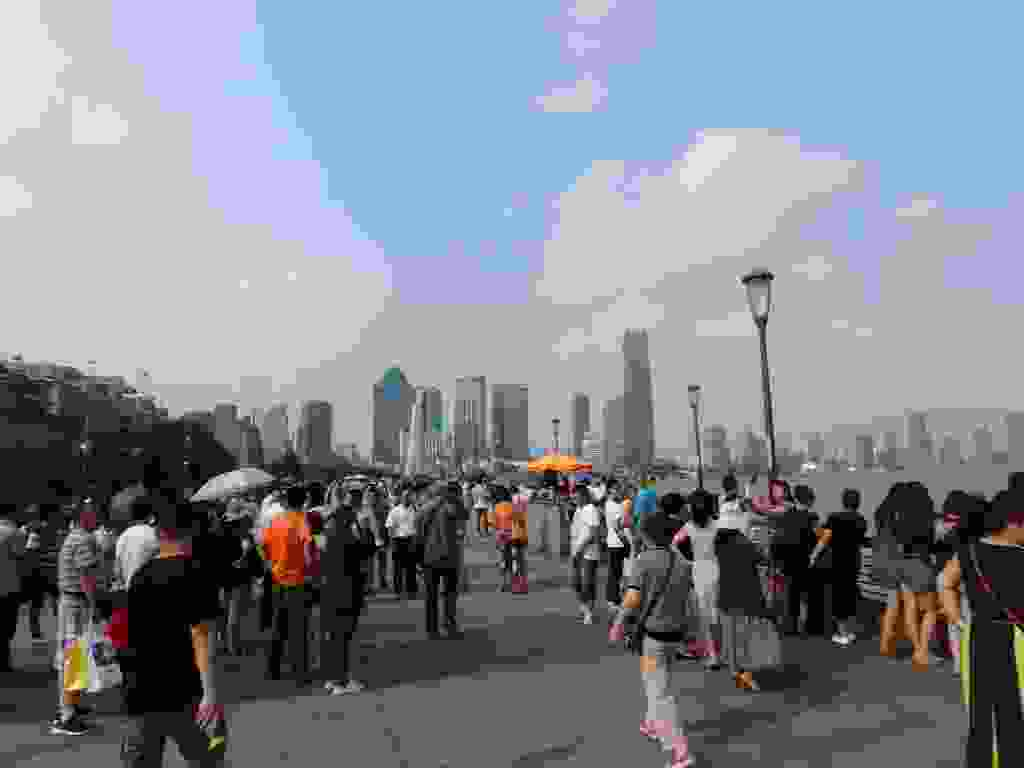
\includegraphics[width=\mywidth]{../wp-content/uploads/2015/09/P8316568-1024x768.jpg} } 
 \newline
 Yuyuan : le quartier traditionnel chinois \newline
 \newline
\centerline{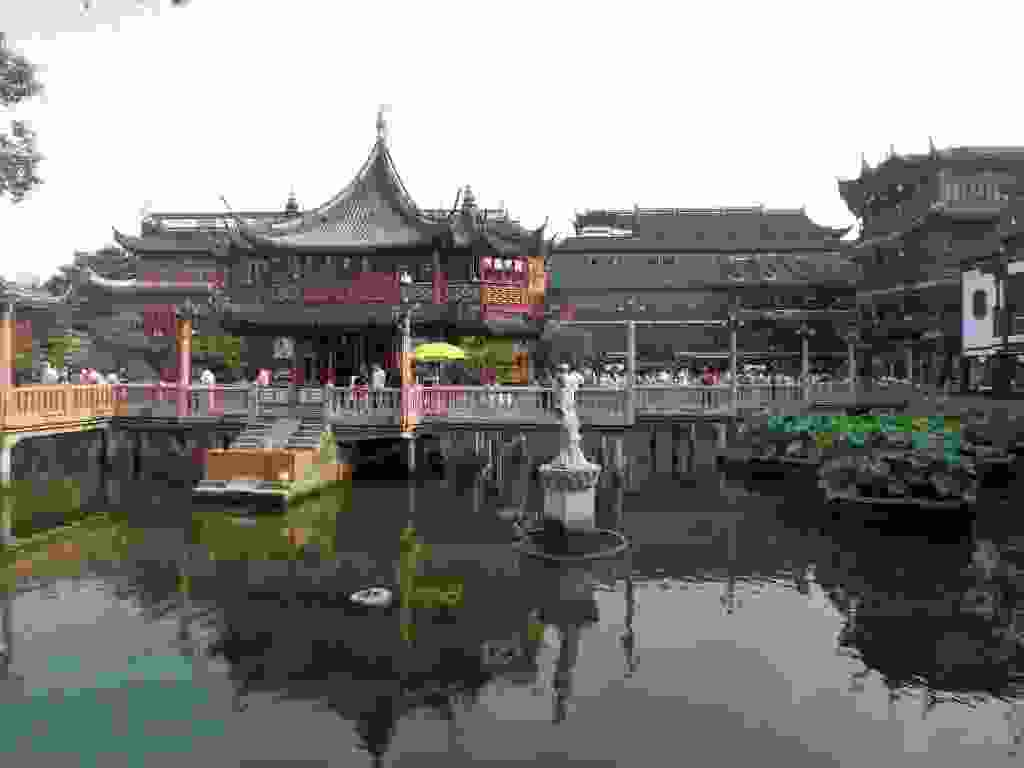
\includegraphics[width=\mywidth]{../wp-content/uploads/2015/09/P8316576-1024x768.jpg} } 
 \newline
 \newline
\centerline{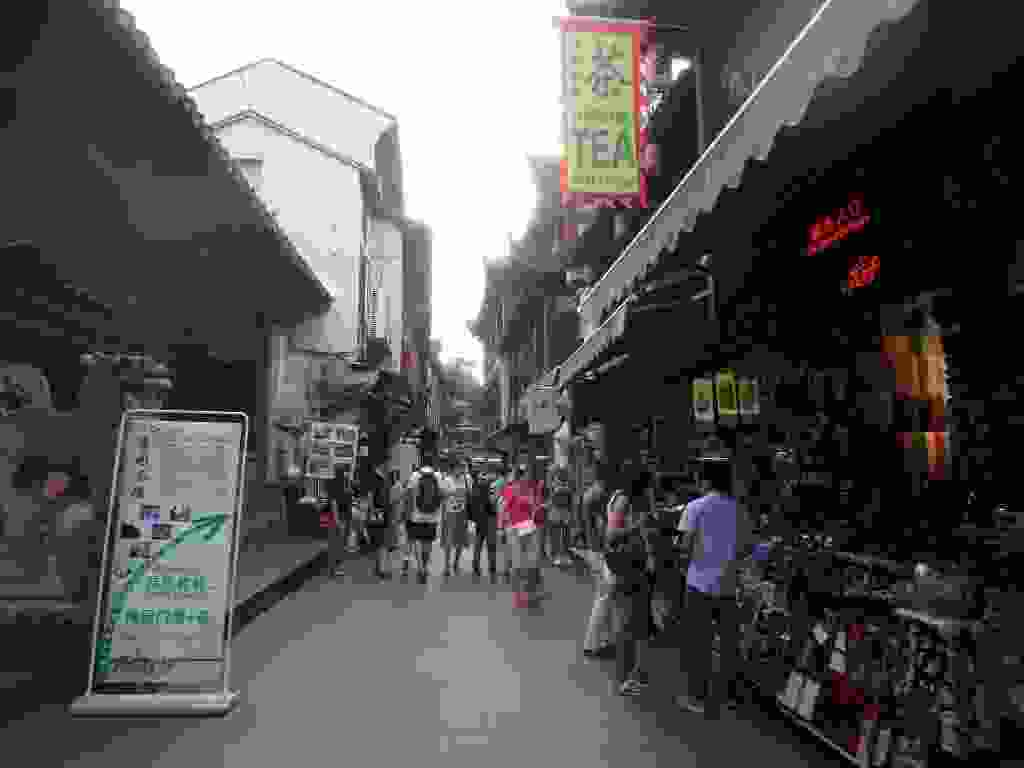
\includegraphics[width=\mywidth]{../wp-content/uploads/2015/09/P8316594-1024x768.jpg} } 
 \newline
 \newline
\centerline{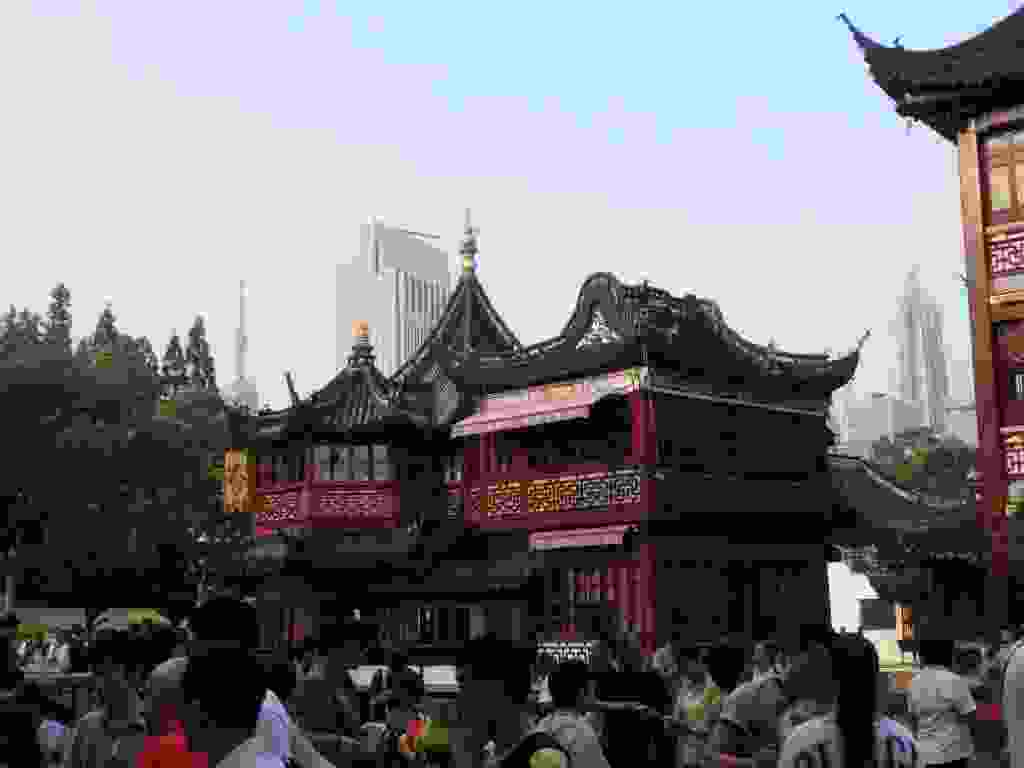
\includegraphics[width=\mywidth]{../wp-content/uploads/2015/09/P8316596-1024x768.jpg} } 
 \newline
 \newline
\centerline{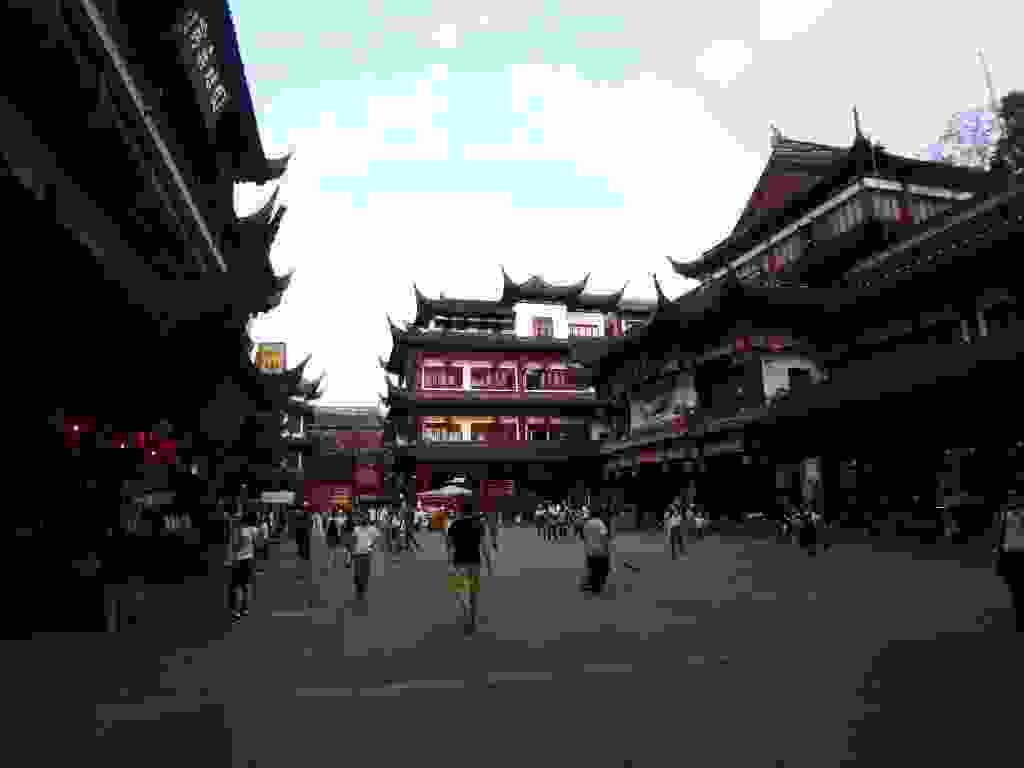
\includegraphics[width=\mywidth]{../wp-content/uploads/2015/09/P8316598-1024x768.jpg} } 
 \newline
 Le jardin Yu avec ses petits pavillons typiques \newline
 \newline
\centerline{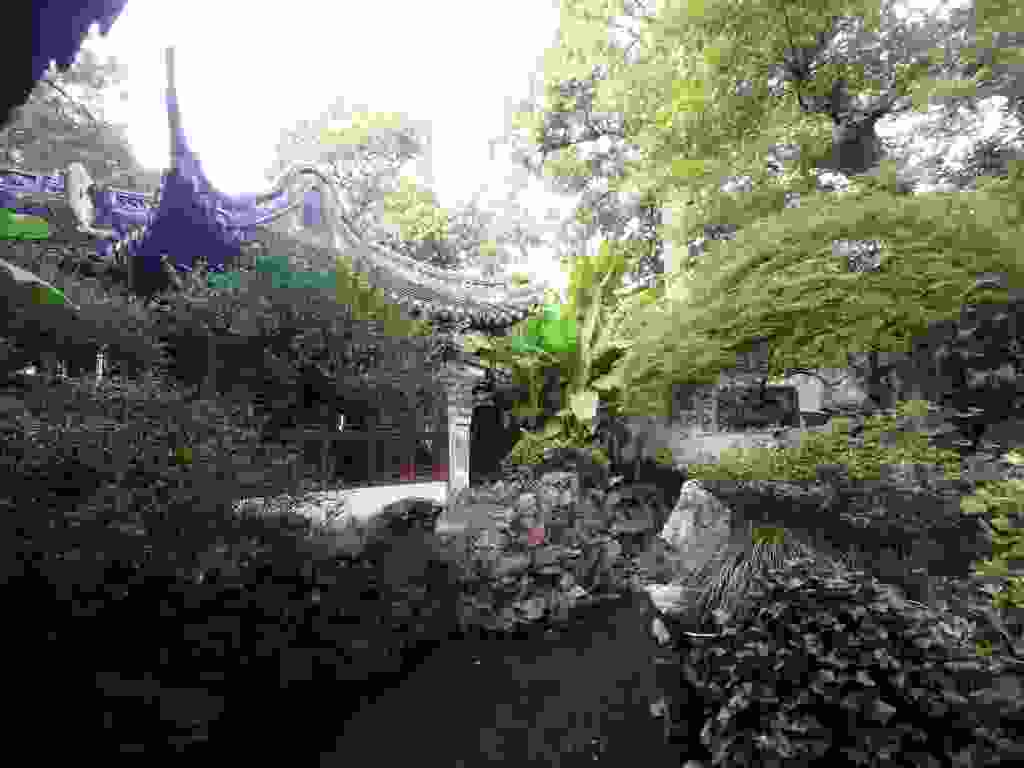
\includegraphics[width=\mywidth]{../wp-content/uploads/2015/09/P8316579-1024x768.jpg} } 
 \newline
 \newline
\centerline{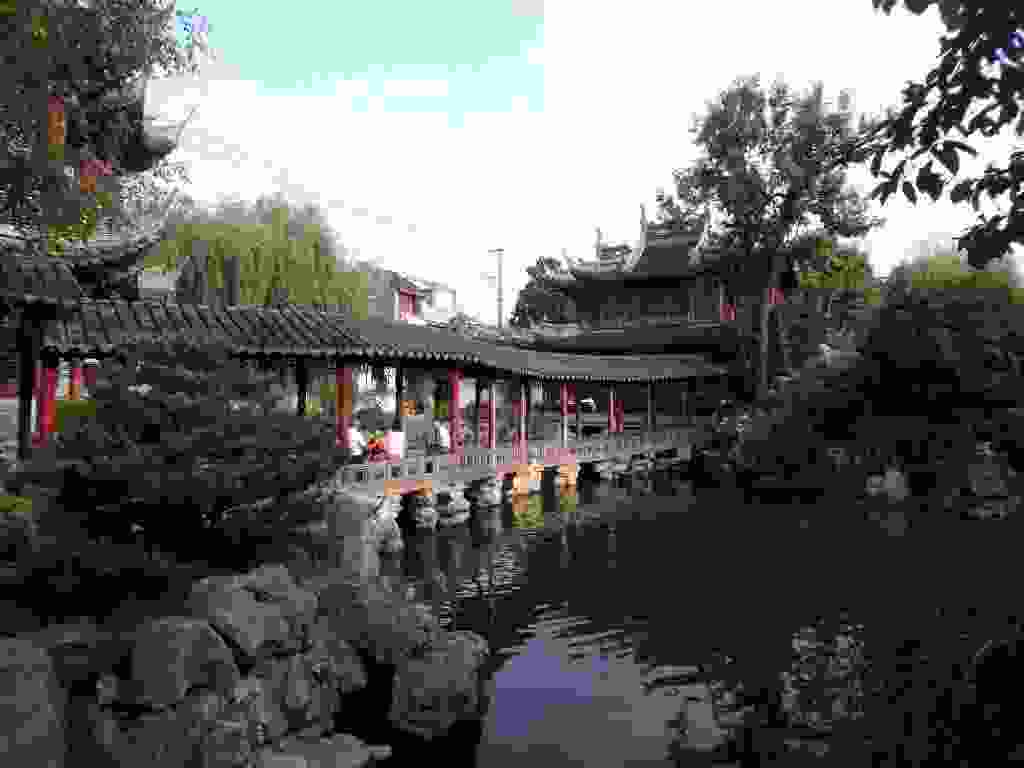
\includegraphics[width=\mywidth]{../wp-content/uploads/2015/09/P8316585-1024x768.jpg} } 
 \newline
 \newline
\centerline{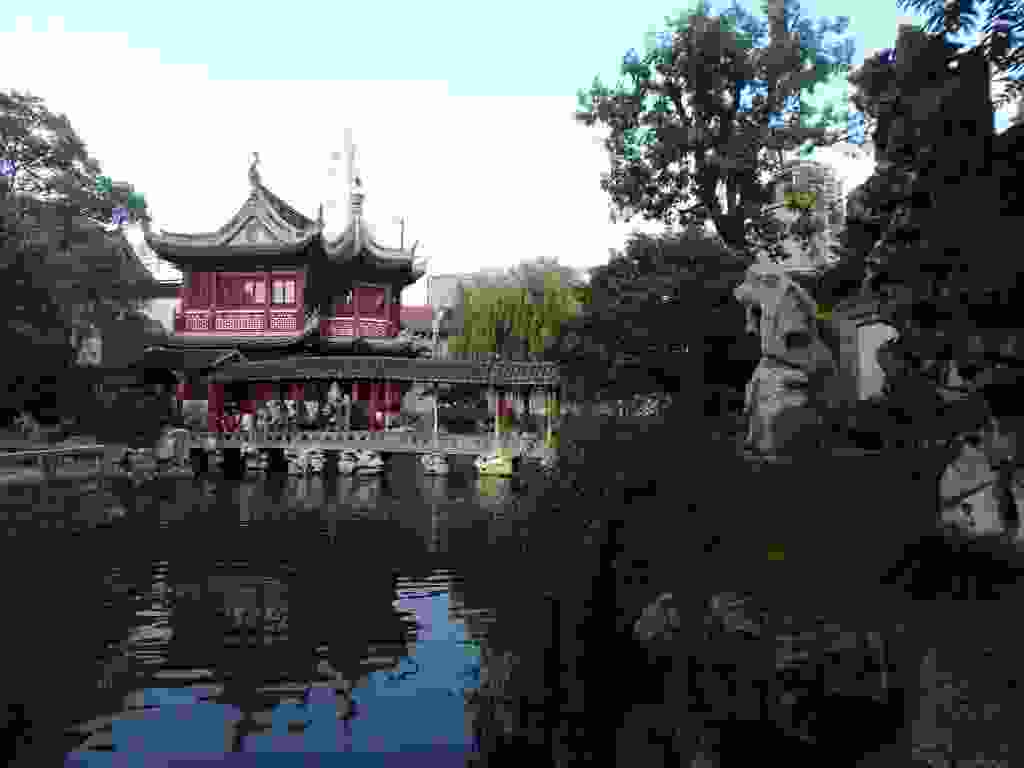
\includegraphics[width=\mywidth]{../wp-content/uploads/2015/09/P8316588-1024x768.jpg} } 
 \newline
 Des animaux sympatiques au marché \newline
 \newline
\centerline{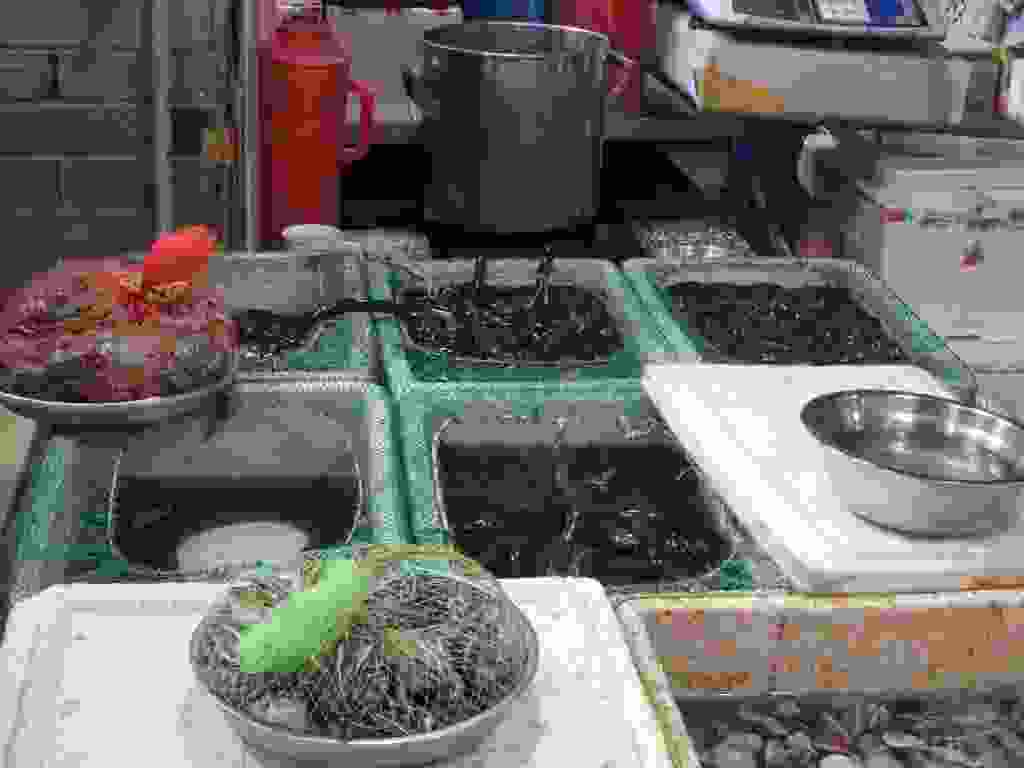
\includegraphics[width=\mywidth]{../wp-content/uploads/2015/09/P9016603-1024x768.jpg} } 
 \newline
 J'ai été accueilli en Warmshowers par Kyle, américain qui organise des visites gastronomiques de Shanghai. Il m'a invité à venir avec sa collègue à une soirée repérage de restaurants, de belles découvertes ! \newline
 \newline
\centerline{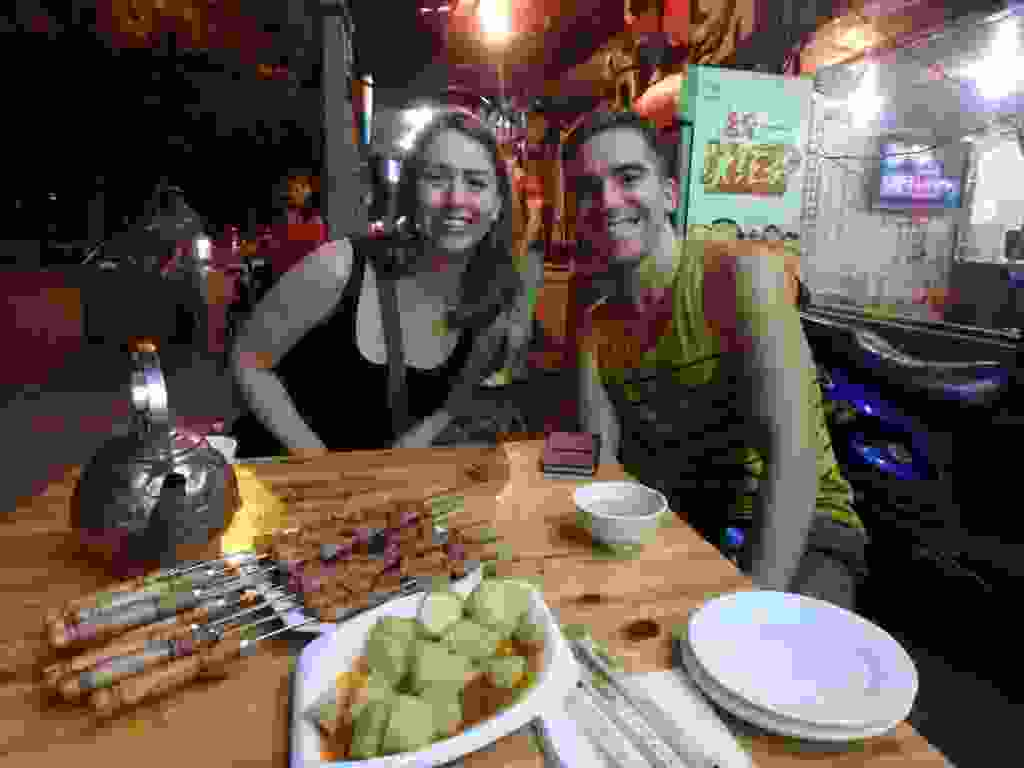
\includegraphics[width=\mywidth]{../wp-content/uploads/2015/09/P9016614-1024x768.jpg} } 
 \newline
 Le ping pong est le sport national en Chine, il faut bien que j'essaye d'aller taper la balle : \newline
 D'abord acheter une raquette chinoise pas chère \newline
 \newline
\centerline{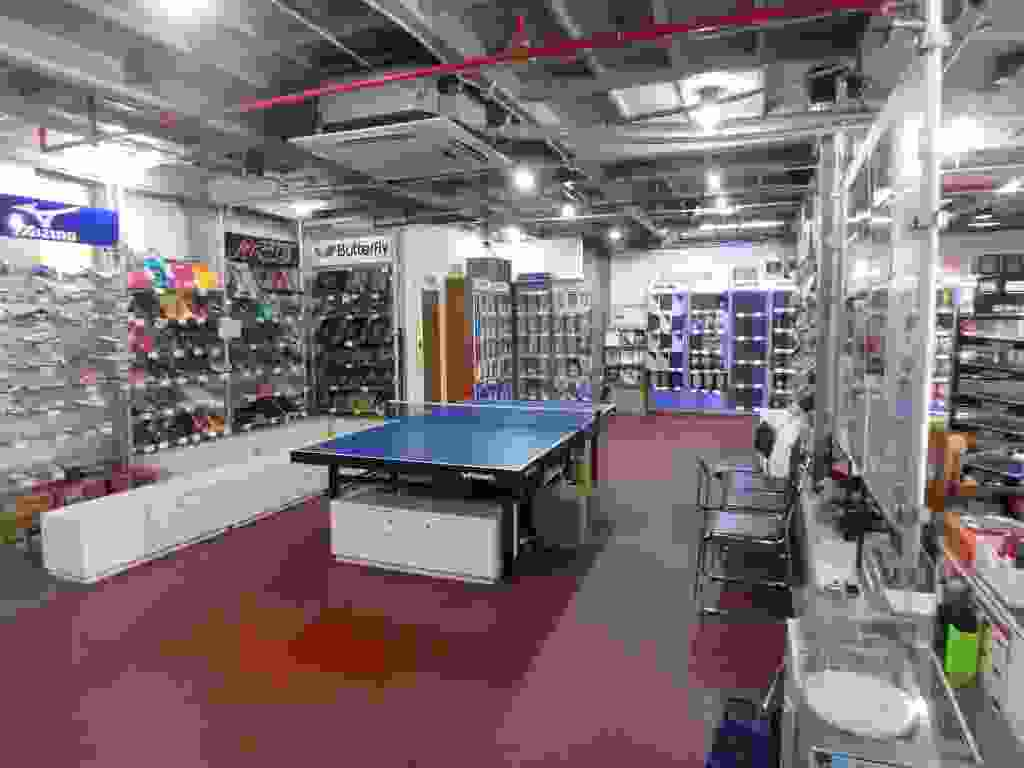
\includegraphics[width=\mywidth]{../wp-content/uploads/2015/09/P9016604-1024x768.jpg} } 
 \newline
 Puis trouver une salle pour jouer un peu, il n'y avait pas trop de monde, bon niveau mais sans plus \newline
 \newline
\centerline{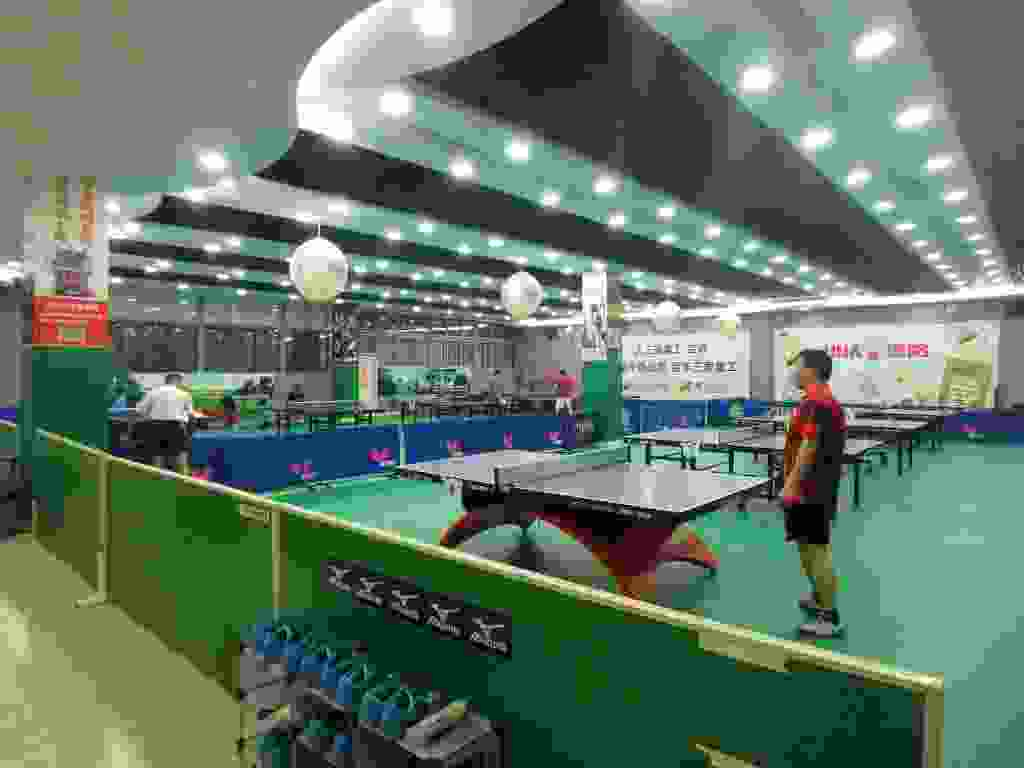
\includegraphics[width=\mywidth]{../wp-content/uploads/2015/09/P9016609-1024x768.jpg} } 
 \newline
 Je quitte Shanghai pour 21h de train direction Xi'an \newline
 \newline
\centerline{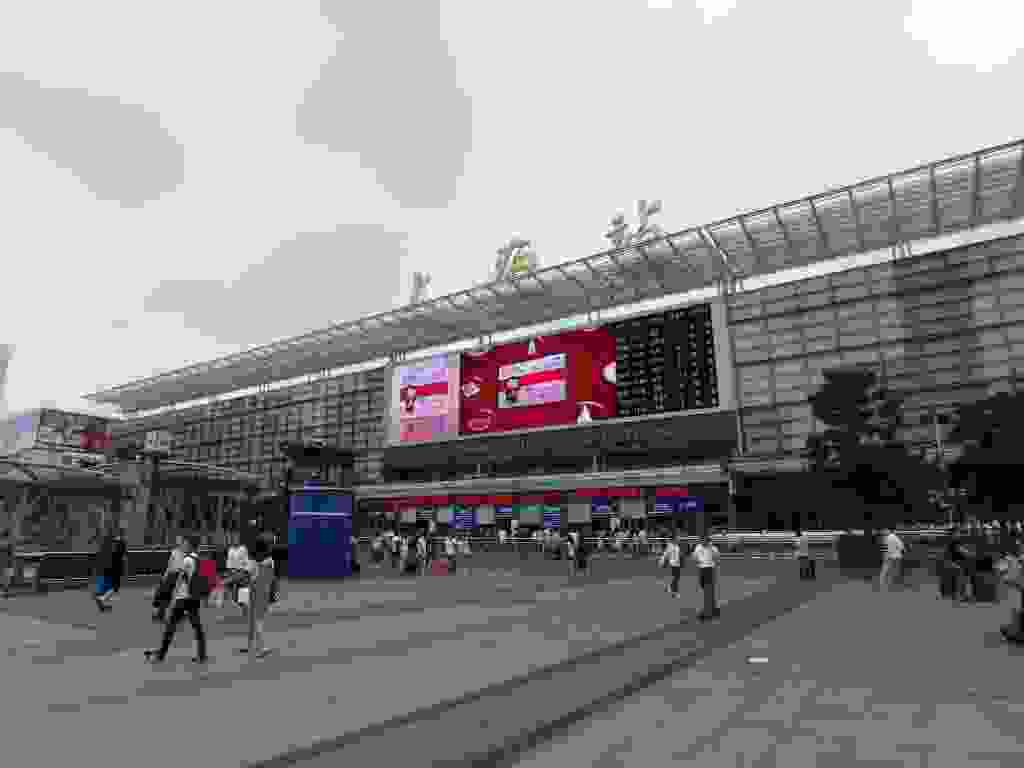
\includegraphics[width=\mywidth]{../wp-content/uploads/2015/09/P8316548-1024x768.jpg} } 
 \newline
 \newline
\centerline{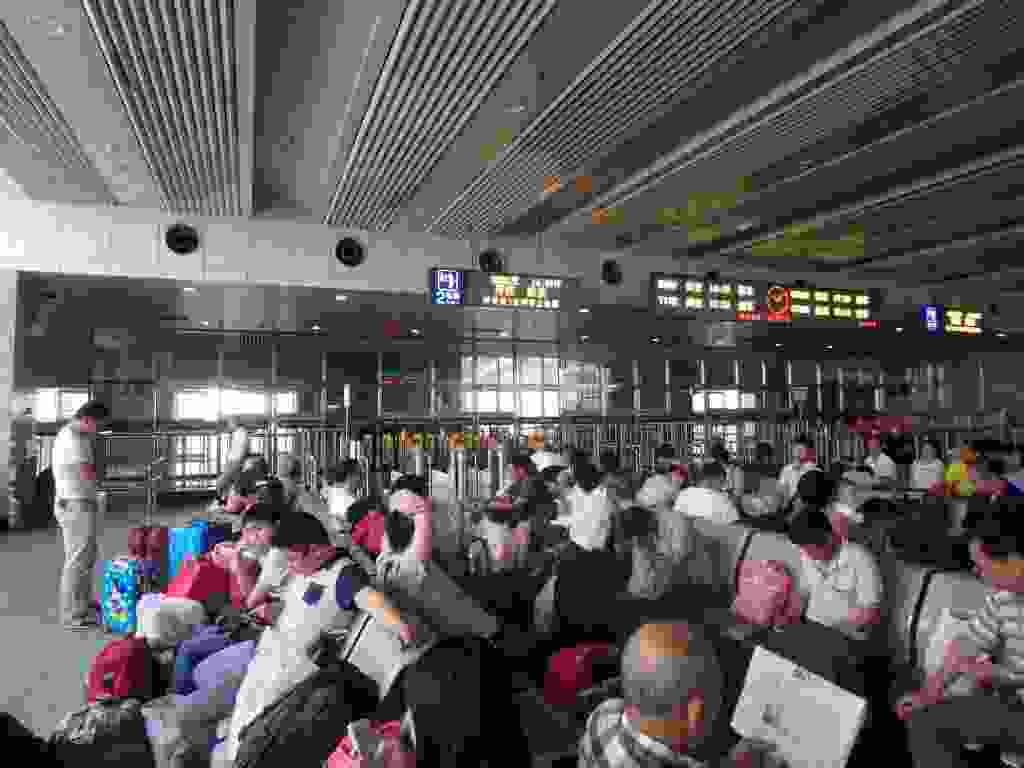
\includegraphics[width=\mywidth]{../wp-content/uploads/2015/09/P9026616-1024x768.jpg} } 
 \newline

\newpage
 
